
\documentclass[a4paper,12pt,notitlepage]{article} % Prepara un report per carta A4, con un font grande 12
 
\usepackage[english]{babel} % Adatta LaTeX alle convenzioni tipografiche inglesi
%\usepackage[T1]{fontenc} % Riga da togliere se si compila con PDFLaTeX
%\usepackage[utf8]{inputenc} % Consente l'uso caratteri accentati italiani
\usepackage[a4paper,top=3cm,bottom=3cm,left=2.0cm,right=2.0cm]{geometry}
\usepackage[superscript]{cite} % i numeri delle citazioni vengono messe in apice nel testo
\usepackage{babelbib} %permette di aggiungere la entry "language" nel database bibliografico
\usepackage[nottoc]{tocbibind} %aggiunge all'indice dei contenuti anche la bibliografia
\usepackage{url} % aggiunge url
\usepackage{hyperref} % aggiunge hyperref nel pdf
\usepackage{graphicx} %non mi ricordo
\usepackage{float} %per gestire la posizione delle immagini
\usepackage{amsmath} %per le formule matematiche
\usepackage{enumerate} %per liste enumerate
\usepackage[noend,boxed]{algorithm2e} % per gli algoritmi
\usepackage{tabu} %non me lo ricordo
\usepackage[format=hang, indention=-2cm,labelfont=bf]{caption} 
\usepackage{changepage} % sposta tabelle
\usepackage{setspace}
\usepackage{fontspec} % permette di cambiare il font
\setmainfont{Calibri}

\onehalfspacing % forza LaTeX ad una spaziatura uniforme, invece di lasciare più spazio
% alla fine dei punti fermi come da convenzione inglese

  
\begin{document}

%\pagestyle{empty}
\begin{center}
	{\bfseries\Huge {UNIVERSITY OF TRENTO}}

	\begin{center}
		
\includegraphics[width=0.2\textwidth]{img/unitn}
	\end{center}
	\vspace{0.5cm}
	{\Large Project of Distributed Algorithms}
	\vspace{0.2cm}

	{ \bfseries \Large {IMPLEMENTATION OF CYCLON OVER THE AKKA FRAMEWORK}}
	\vspace{2.0cm}
	\large
	\begin{center}
		\begin{tabular}{lcl}
			%Relatore: & \hspace{5cm} &  Graduant: \\
			Luca Zamboni & \hspace{5cm} &  Luca Erculiani \\
			XXXXXX & \hspace{6cm} &  XXXXXX \\ \\
%			luca.zamboni@unitn.it & \hspace{4cm} &  luca.erculiani@unitn.it \\
		\end{tabular}
	\end{center}
	\vspace{1.0cm}
\end{center}
\begin{abstract}
   	 	
    The topic of this work is the implementation of Cyclon, a decentralized
    peer-to-peer protocol for gossiping over the Akka framework \cite{Akka}.
    The goal of Cyclon is to build a network that can resist against crash of 
    a great part of its node without  collapsing in a series of disconnected clusters.
    This document will explain first the theoretical basis of the protocol, then 
    our implementation of a program capable of simulating a Cyclon network. 
    The last part of this work will be focused on the statistical
    result of simulations made, discussing the capabilities of the network
    to build a strongly connected graph, to resist to massive disconnection. The 
    last test will show the limits of the protocol in case of hub attack.
  

\end{abstract}
\newpage


% \pdfbookmark{\contentsname}{toc}
% \tableofcontents % Prepara l'indice generale
% \newpage

\section{INTRODUCTION}

The goal of this work is to implement a simulation of a peer-to-peer network running
 the Cyclon gossiping's protocol, for the project of Distributed Algorithms, by Alberto Montresor. 
 The network is strongly decentralized and consist in a 
 large number of peer clients and one or more tracker server, whose function is to allow new 
 peers to connect into the network. Now will follow a list of descriptions of the topics of every
 section of this document.

 \begin{itemize}
 	\item The system model section will describe the Cyclon protocol, showing  the general structure of 
 	the algorithms that implement it and focusing on the particular elements that characterize it.
 	\item The implementation section is focused on explaining the actual implementation of 
 	our simulation, discussing about the choices made by development and the input and
 	 output of the program.
 	\item The analysis and result section will show informations about tests executed on 
 	the program, for evaluating some characteristic of Cyclon
 \end{itemize}



\section{SYSTEM MODEL}

The system that we want to model is a dynamic collection of distributed nodes that wants to participate in
 a epidemic protocol. The number of node isn't fixed and can increase or decrease depending on peers who
 join and leave the protocol, or maybe crash. 
 The communication between pairs of nodes needs that one 
 of them knows the address of the other one, and the channel is a best-effort type (potentially a lot of 
 message omission). 


\subsection{SERVICE SPECIFICATION}

Nodes has only a partial views of the network, and this view is dynamic. Each node periodically 
 gossip with a random neighbour about its other neighbour. The main idea is that nodes continuously
 exchange information about other nodes, removing the old ones (so the most probable disappeared) and
 adding the new ones. Each node has a fixed number of neighbour and shuffle this with other nodes.
 For communicating with another node, a peer needs a neighbor descriptor of that node, consisting:

 \begin{itemize}
 	\item the address of that node
 	\item a timestamp information about the age of the descriptor
 	\item more additional information, maybe needed by the upper software layer\cite{slideMontre}
 \end{itemize}

When a new node want to enter in the protocol asks to a tracker 
 server a random subset of peers and starts the communication.

 \subsection{SKELETON OF THE ALGORITHM}	
Here is presented the structure of the code of an instance running Cyclon. The algorithm
 is common to a bunch of protocol with the same purpose, like Newscast\cite{newscast}.


\begin{algorithm}[H]
\SetAlgoLined
\SetKwProg{Upon}{upon}{ do}{end}
\SetKwProg{UponRec}{upon receive}{ do}{end}
\SetKwProg{Repeat}{repeat}{ }{end}
\SetKw{Send}{send}
\SetKw{To}{to}

\Upon{inizialization}{
	\(view \leftarrow\) descriptor(s) of nodes already in the system
	}
\BlankLine
\Repeat{every \(\Delta\) time units}{
	Process \(q \leftarrow\) selectNeighbor(\(view\))

	\(m \leftarrow\) prepareRequest(\(view,q\))

	\Send \(\langle\mbox{REQUEST},m,p\rangle\) \To{q}
	}
\BlankLine

\UponRec{\(\langle\mbox{REQUEST},m,q\rangle\)}{
	\(m \leftarrow\) prepareReplay(\(view,q\))

	\Send \(\langle\mbox{REPLY},m',p\rangle\) \To{q}

	\(view \leftarrow\) merge(\(view,m,q\))
}
\BlankLine

\UponRec{\(\langle\mbox{REPLY},m,q\rangle\)}{
	\(view \leftarrow\) merge(\(view,m,q\))

}
\BlankLine
\end{algorithm}

What make every protocol different is the behaviour of
 the three functions called in the previous pseudocode. In Cyclon these components acts
 in this way:

\begin{itemize}
	\item selectNeighbor() selects the oldest neighbor in the view
	\item prepareRequest(\(view, q\)) removes \(t-1\) random descriptors from the view and return this 
	subset plus a fresh local one
	\item prepareReply(\(view, q\)) removes and return t freshest neighbors from the local view
	\item merge(\(view, m, q\)) merges the local view and the one received, if there are duplicates keeps only the 
	freshest. Removes itself and reinsert entries sent to \(q\) if space permits
\end{itemize}






\section{IMPLEMENTATION}

We have implemented protocol Cyclon with Akka framework in Java.
We have choosen Akka because it offers a really good scalable Peer simulator and easy manage interface messages exchanging.

\subsection{MESSAGE}
	There are two type of message in our Project. When a Peer is 	created it sends a message of type Message.java to 
the tracker it contains only the information about the sender and nothing else. The other message of type MessagePeer.java 
contains the sender of the message and the list of Peer that you are exchanging and also the type of the message. 
MessagePeer.java can take different values:
\begin{itemize}
  \item 0 If it is the response of the Tracker.
  \item 1 If a Peer start an exchange sending some Peer to another Peer.
  \item 2 If it is a response for another that sent some Peer.
  \item -1 If this Peer is Died. This is only to simulate a dead peer.
\end{itemize}

\subsection{TRACKER}
	Tracker.java has the task to give some address of peers to a Peer that has been created. It receives a Message of 
type Message.java from the Peer, it subscribe the new Peer to the local List of Peers in the network. After that it chooses 
\(n\) newest Peers in the list and sends it back to the Peer a message that contains the list.

\subsection{PEER}
	This is the main class of the project. It simulates a Peer in the network. This class has the following structure:  
\begin{itemize}
\item preStart(). Basically requests the peer from tracker sending a Message.java and subscribes this peer to the monitor 
 for get data for statistic.
\item onReceive(Object message). This function handles messages. If type is 0 is just  itializes the list of neighbors. If 
type is 1 it sends a message of type 2 with his \(n\) neighbors plus him. After reply it merges the 
received Peers. If type is 2 it just merge the received Peer from the sender. If the type of the message is -1  removes the 
sender from his neighbors.
\item merge(int type, ArrayList<Peer> peers). Is a function that merges peers with local neighbors and if the size of the 
list remains under the minimum size it fills with older neighbors known in the previous cycle.
\item send(int type, Peer to). If the type of the message is 1 it choose n-1 random peer. If it is 2 it choose last n peer 
with higher timestamp. After this it sends the chosen peer to the Peer.
\item selectPeerToContact() selects the neighbor with lower timestamp.
\item run() waits DELTA time to restart a cycle.
\item removeNodeFromNeighbors(Peer peer). Removes peer from list neighbors.

\end{itemize}

\subsection{COLLECTING DATA}
	When a Peer is initialized he subscribes itself to the monitor. The monitor every DELTA seconds writes on file the 
neighbors of every peer with the average of the  number of cycle and start a GUI that shows the evolution of the 
neighbors of peers.

\subsection{SIMULATION}
	When a Peer is created it subscribes itself to the monitor  just to collect data for statistics. After it sends a 
request the initial list of Peers to the Tracker. The Tracker writes it to the global list of peers in the system and sends 
back the subset of the newests in the network. The peer now starts first cycle of his life. It selects the peer with older 
timestamp and sends him his n-1 random neighbors with himself added to the list with a fresh timestamp. The peer that receives 
the message selects his older n neighbors and sends it back to the sender and merge those who arrived with its local 
neighbors. Now the peer that started the request receives the list of peers and merges it with is's local view of the network 
and after that it starts a new run after DELTA time. Every n second monitor writes on file the list of neighbors of each 
peer.





\section{ANALYSIS AND RESULTS}

In this section we will discuss the results of simulations over the implemented protocol and some tests done under
 partarticular conditions.

\subsection{ANALYSIS METHODS}

The output of the program was used to build  graphs, using the NetworkX libraries\cite{netwx} in Python, where
 nodes are peers and edges are the neighbors of every peer. We used undirected graphs except for the 
 computations of in-degrees, where we obviously built a directed graph with direction peer \(\rightarrow\) neighbor.
 The switch to a graph structure allowed a series of operations, like the count of the connected components (or clusters), 
 needed to interpret the shape of the network.

We approximated a couple of operation on the graph, in order to be able to execute it in a reasonable time. In 
 particular the computation of the clustering coefficient was made using a function of NetworkX that make an 
approximation. The average path length was approximated computing the average path length of a number 
\(n\) of random couples of nodes.



\subsection{GENERAL TESTS}

In these tests we executed the simulation without interfering during the run, so no crashes or 
 communication failures were induced. This simulations were done building a network of 20.000 
 peers with 20 neighbors and 10 of them exchanged at every cycle. In every simulation the Cyclon
 graph is compared to a graph with the same number of nodes and the same number of edges randomly distributed.

The first simulation  (figure \ref{avg}) compares the approximated average path length of the two graphs. We can 
 see that after few cycles the avg becomes comparable with the one of the random graph. This is the 
 optimum result in a network fully decentralized without a hierarchy.

\begin{figure} [H]
	\centering
	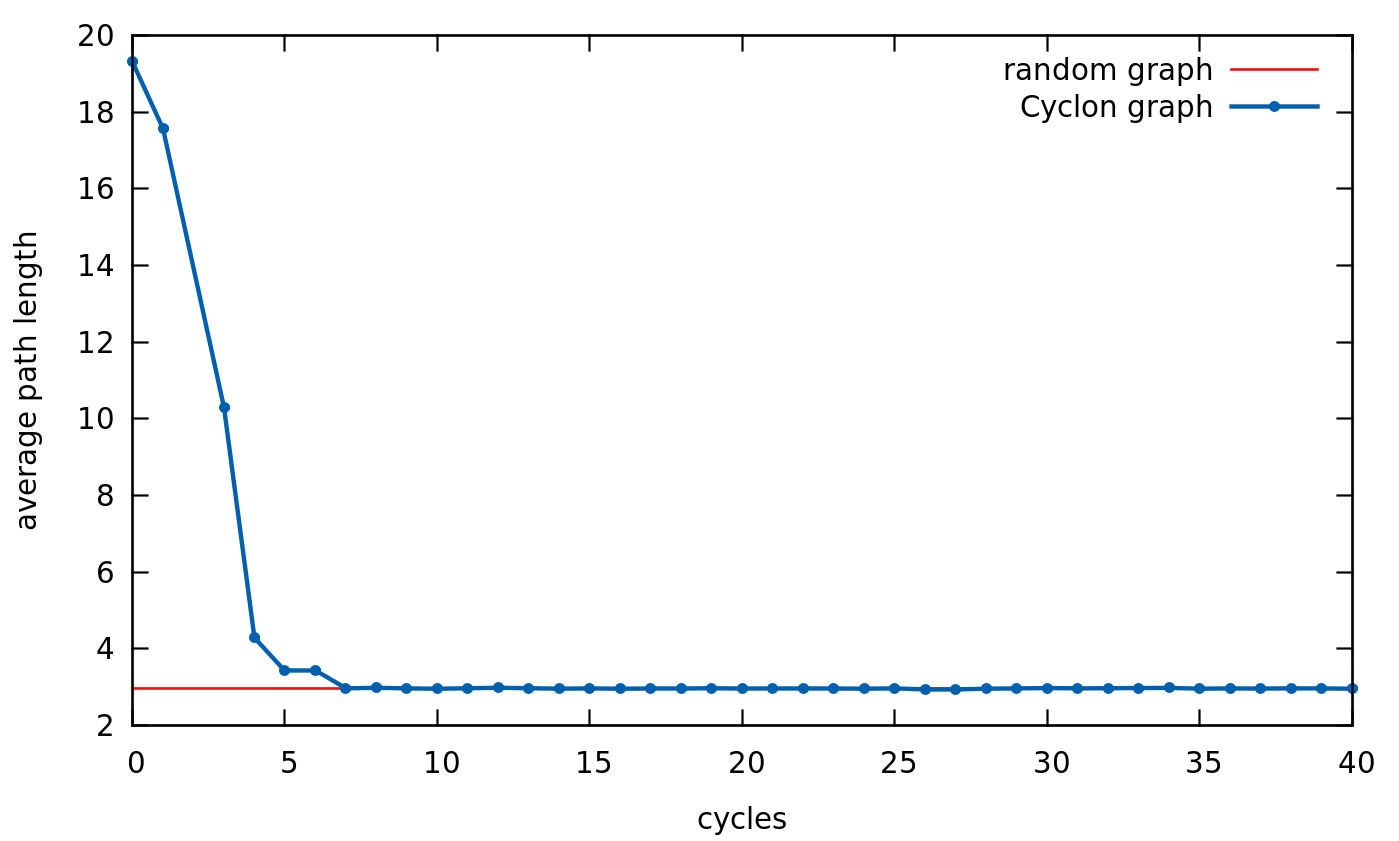
\includegraphics[width=1\textwidth]{img/avgplen}
	\caption{Average path length of random graph and Cyclon graph through  cycles }
	\label{avg}
\end{figure}


The figure \ref{deg} shows the in-degree nodes distribution for the Cyclon and the random graph.
 The results show how the Cyclon graph has more nodes near the mean (20) than the random graph.

\begin{figure} [H]
	\centering
	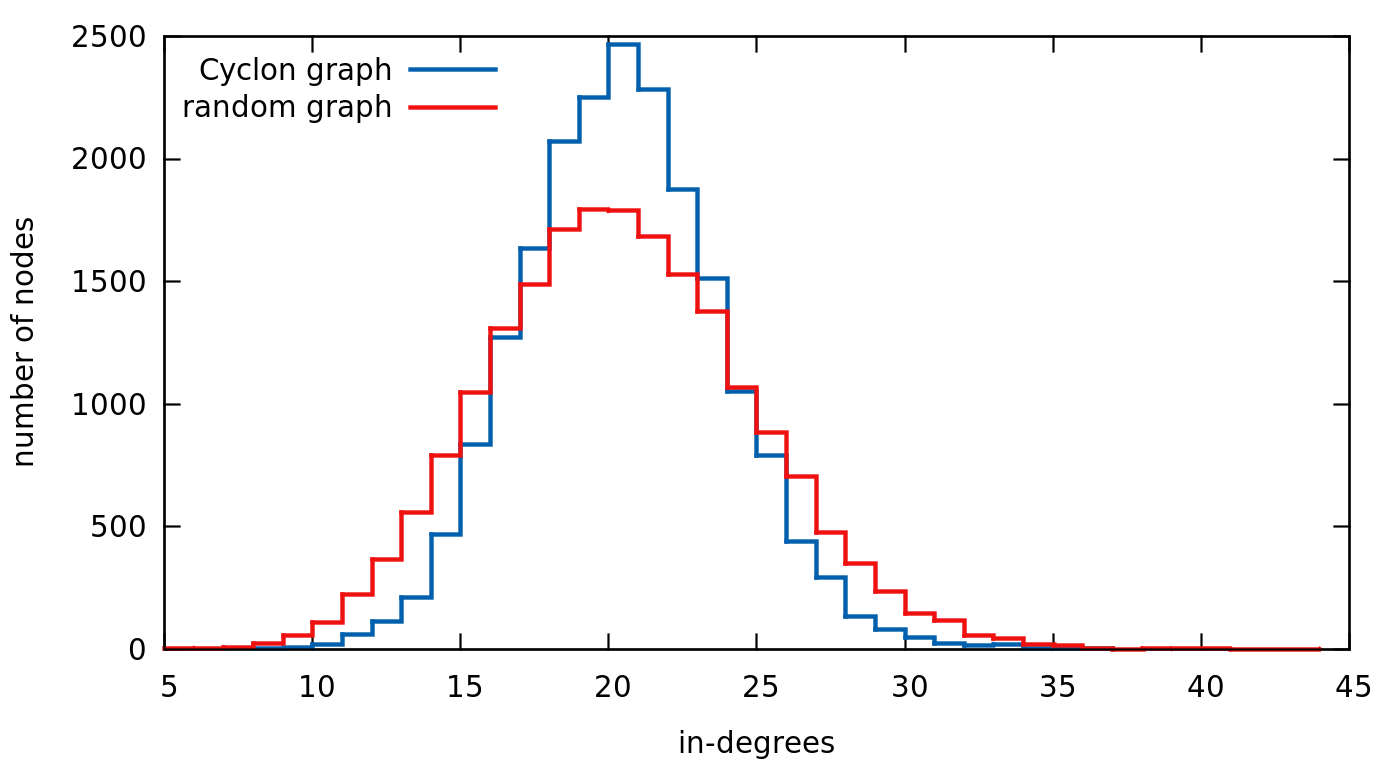
\includegraphics[width=1\textwidth]{img/Degrees}
	\caption{In-degree distribution for Cyclon and random graph}
	\label{deg}
\end{figure}


\subsubsection{ROBUSTNESS TESTS}
These simulations want to show the robustness of the Cyclon protocol, that means its non
 hierarchical structure, that prevents damage in case of disconnection because there aren't
 fundamental peers for the network, and the resistance to massive node disconnection.

The first simulation (graph \ref{clust}) regards the variation of the approximated clustering coefficient. The network,
 after few cycles, reaches the levels of the random graph. This is considered an index of robustness of the 
 network, because of it means that there aren't nodes more important (significantly connected) than others.

\begin{figure} [H]
	\centering
	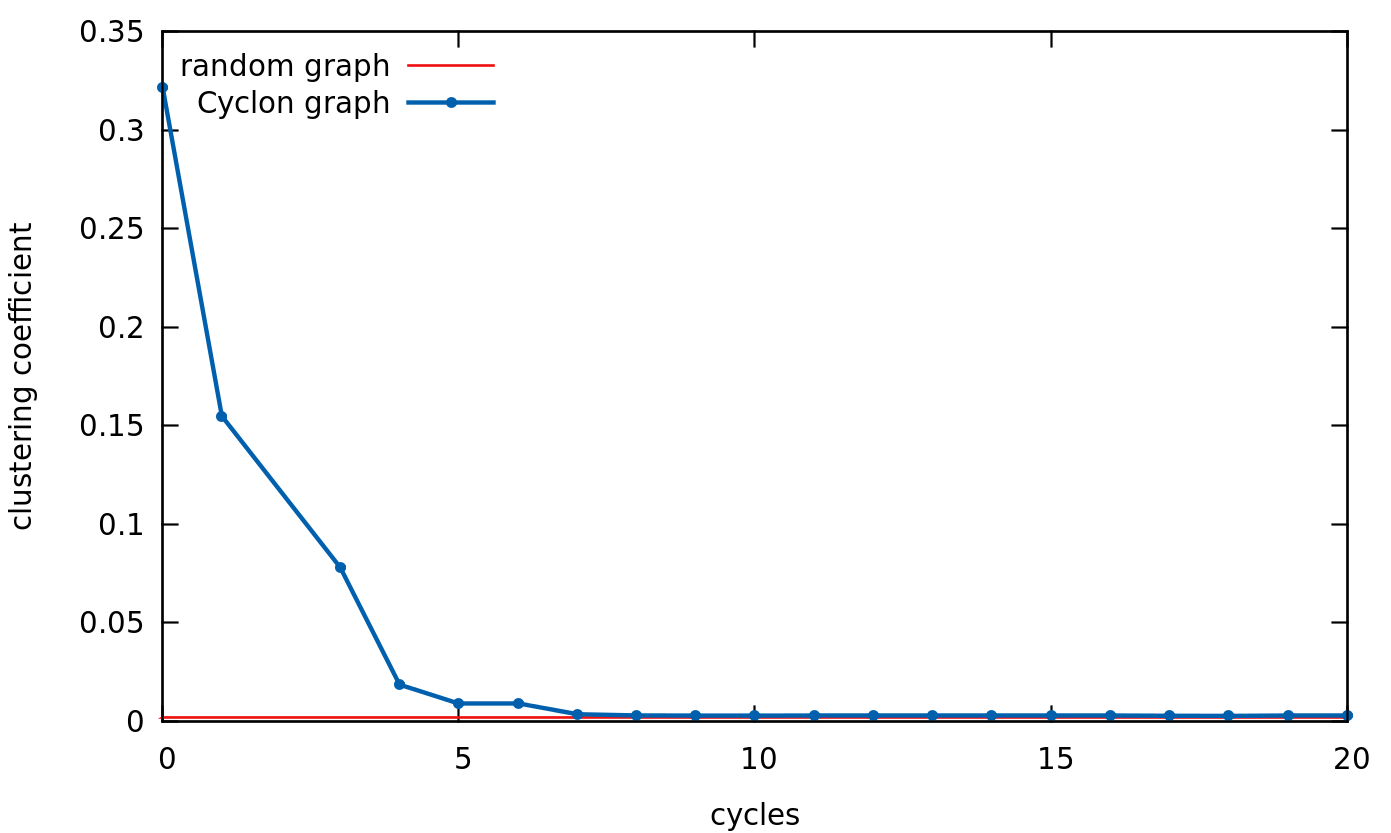
\includegraphics[width=1\textwidth]{img/clustering}
	\caption{Clustering coefficient of random graph and Cyclon graph through  cycles }
	\label{clust}
\end{figure}


Another robustness test is the count of the connected components of the graph after the removal of a certain 
 percentage of nodes in the network. For every percentage tested we repeated for 10 times the removal of the
 nodes and made an average of the clusters generated. The graph \ref{robust} shows how the network remains
 connected until more than three quarters of nodes were removed, obtaining results comparable to the random
 graph.
 
\begin{figure} [H]
	\centering
	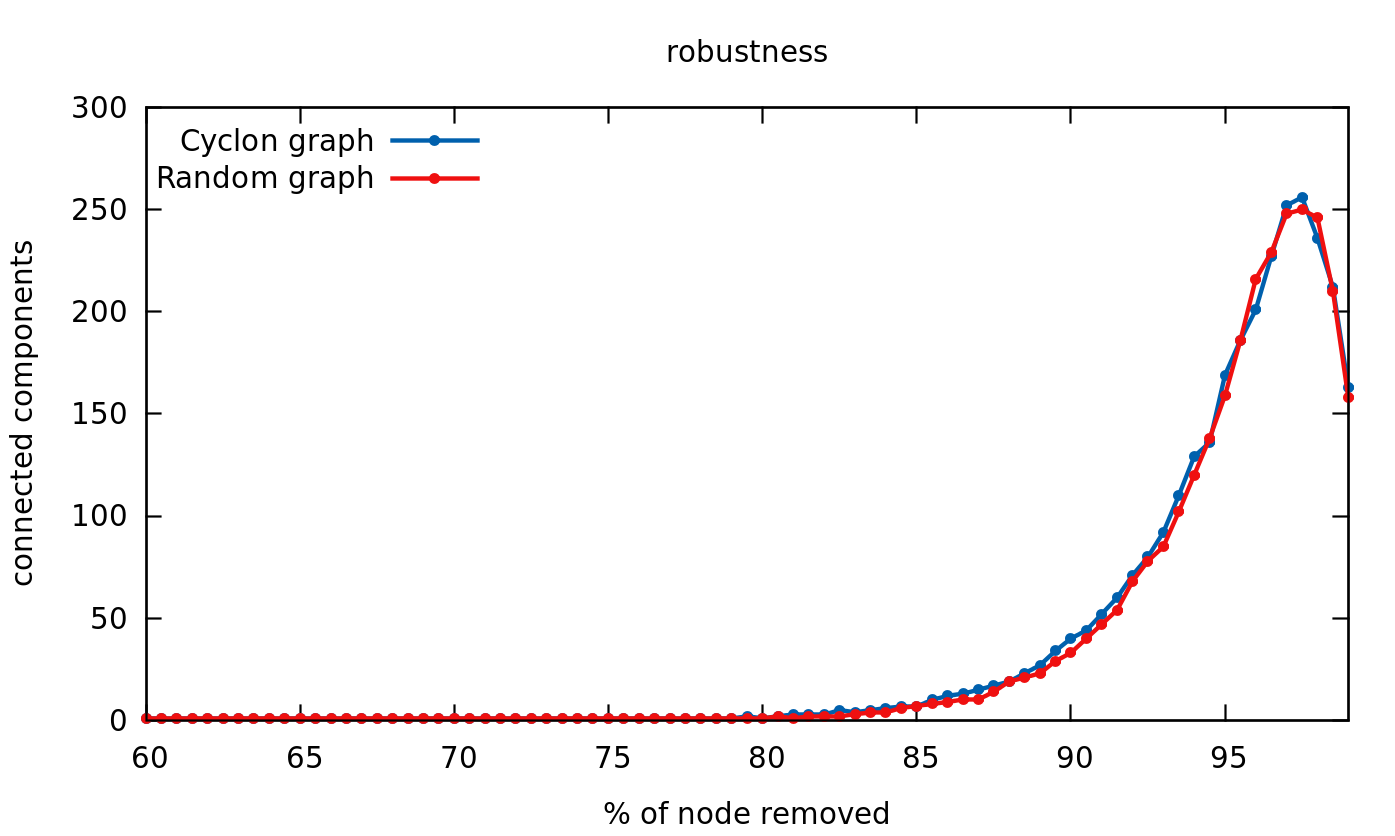
\includegraphics[width=1\textwidth]{img/robustness}
	\caption{Connected components created by removing certain percentages of nodes in Cyclon and in the random graph}
	\label{robust}
\end{figure}

 \subsection{LIVENESS TESTS}

Another important feature requested to this type of protocols is the ability of maintain their network
 alive and free of garbage (references to peers still not present). We executed these tests with three different 
 simulation varying the parameters of the neighbors kept and exchanged. The network had 5000 peers and
 20-15-15 neighbor kept and 10-7-5 exchanged every cycle.

The first test was the ability of self-cleaning. The results (fig \ref{sc}) show that the less number of neighbors
 allows the network to forget of the dead peers faster. The number of neighbor exchanged seems influence
 the speed of the process, in the sense that increasing the number of exchanged decrease the cycles needed
 for clean the network.

\begin{figure} [H]
	\centering
	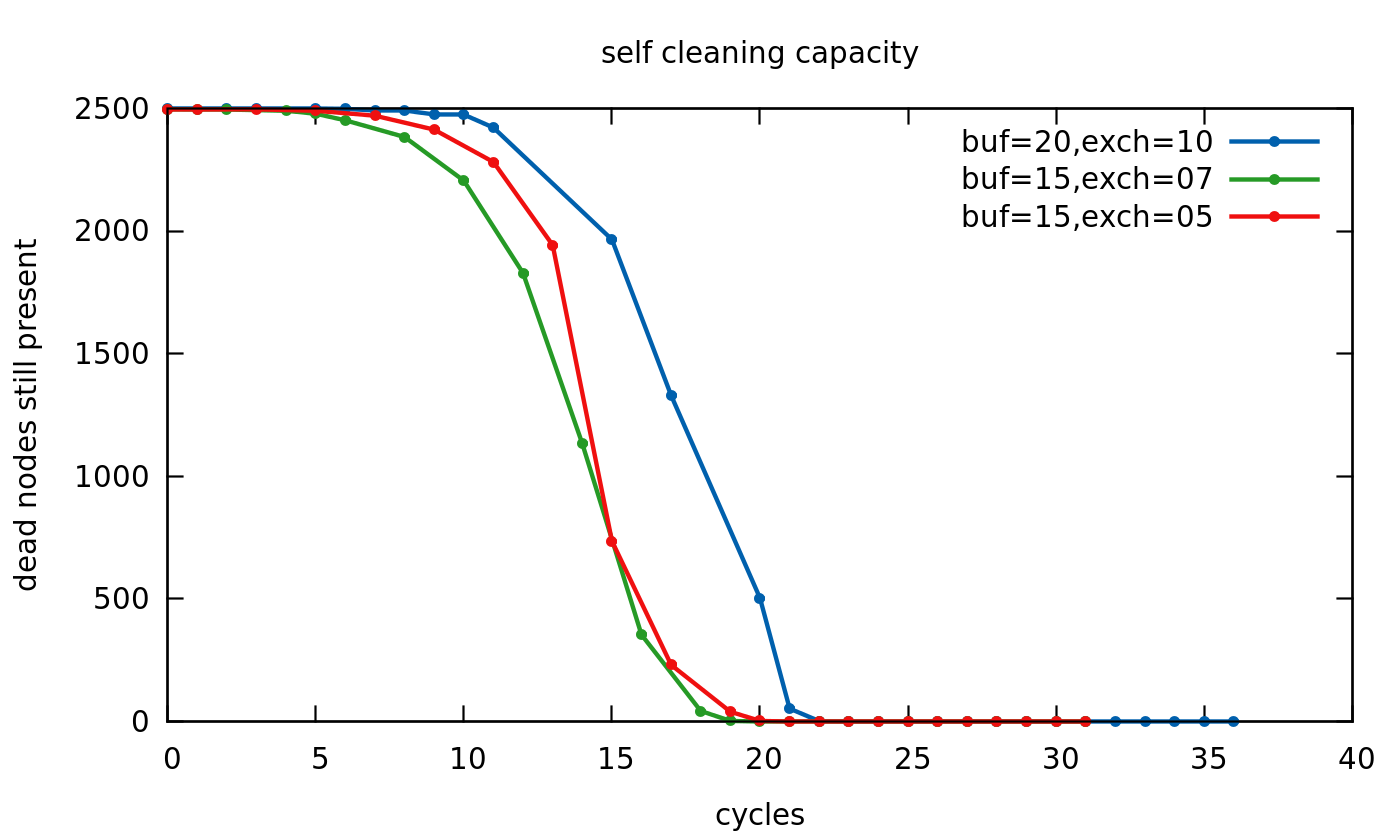
\includegraphics[width=1\textwidth]{img/self_cleaning}
	\caption{Number of cycles required to delete 2500 dead nodes}
	\label{sc}
\end{figure}

The last test executed was an hub attack test. We created 50 peers that exchanged only themselves, and measured
 at the end of every cycle the number of clusters after the removing of the malicious peers. As the 
 figure \ref{attack} shows, the simple Cyclon protocol cannot resist and becomes polluted after few tens of cycles.

\begin{figure} [H]
	\centering
	\includegraphics[width=1\textwidth]{img/attack}
	\caption{Number of clusters created at every cycle by 50 malicious peers}
	\label{attack}
\end{figure}


% \subsection{CONCLUSIONS}
% The tests executed on the network showed that the implemented simulation respects all the expectations
%  of a standard Cyclon protocol. The execution 

\begin{thebibliography}{9}

\bibitem{Akka}
  The Akka framework,
  \url{http://akka.io/}

\bibitem{slideMontre}
  Distributed Algorithms course,
  Montresor Alberto,
  slide ``epidemics2'',
  \url{http://disi.unitn.it/~montreso/ds/slides.shtml}


\bibitem{newscast}
  A Robust and Scalable Peer-to-Peer Gossiping Protocol by
  Spyros Voulgaris, M´ark Jelasity and Maarten van Steen,

\bibitem{netwx}
  NetworkX,
  \url{https://networkx.github.io/}



\end{thebibliography}







\end{document}

